% Chapter Three: Methodology
% Compiled through Opol_Charis_Thesis.tex; do not compile this file on its own.

\chapterheading{THREE}{METHODOLOGY}

This chapter describes how the study will be carried out. It presents the research design and the pipeline of the project, and then describes each component in turn: the modelling of incident scenarios, the simulated triage environment, the reinforcement learning agent, the rule-based safety mechanism and the baseline decision policies. It then defines the evaluation metrics and the experiments, and closes with the tools, the threats to validity and the ethical considerations of the study. The chapter describes planned work, and it reports no results.

\section{Research Design}

The study follows a design-and-evaluate approach. It constructs an artefact, a rule-constrained reinforcement learning agent together with the environment in which the agent operates, and it evaluates that artefact through controlled experiments. This corresponds to the design science view of research in information systems, in which knowledge is produced by building an artefact that addresses an identified problem and by evaluating it rigorously~\cite{hevner2004}. The design suits the research questions, which ask how a task can be represented, how a method can be applied to it, and how well the result performs.

The evaluation is experimental and quantitative, and it is conducted entirely in simulation. Chapter Two showed that realistic incident data is scarce and confidential and that simulation is the accepted response in studies of sequential decision-making for incident handling~\cite{remil2024,hammar2025,dunsin2025}. Simulation also gives the study control over the variable of interest. The level of ambiguity can be set, held constant and varied, which would not be possible with live incidents. The cost of this choice is that the findings describe the behaviour of the agent under the assumptions of the simulator, a limit that Section~\ref{sec:validity} discusses.

A qualitative component informs the simulation. The Directorate of University ICT Services at Uganda Christian University has agreed to support the study, and its practice is the source from which the incident scenarios and operational rules are drawn. An initial semi-structured interview with a senior developer of the Directorate, held on 19 October 2026, described the current handling of incidents: users or support staff raise tickets, which are vetted and assigned to the responsible developer or, where that person is not known, to a senior developer; application errors are observed through system logs and a monitoring dashboard. The interviewee identified the application programming interface logs as the most informative source of evidence. This consultation shaped the incident categories in Section~\ref{sec:scenarios} and the treatment of escalation as a hand-over to the responsible member of staff. Table~\ref{tab:alignment} shows how each specific objective is addressed by a component of the method and by a set of measures.

\begin{table}[htbp]
\centering
\caption{Alignment of the specific objectives with the method and the evaluation.}
\label{tab:alignment}
\small
\begin{tabularx}{\textwidth}{@{}p{0.27\textwidth}LL@{}}
\toprule
Objective & Method component & Evidence produced \\
\midrule
1. Identify and model ambiguous triage scenarios & Scenario elicitation and incident model (Sections~\ref{sec:scenarios} and~\ref{sec:environment}) & Scenario model reviewed by Directorate staff \\
2. Design the reinforcement learning environment & Simulated triage environment and agent (Sections~\ref{sec:environment} and~\ref{sec:agent}) & Working environment; learning curves \\
3. Implement the rule-based safety mechanism & Safety mechanism (Section~\ref{sec:mechanism}) & Constraint compliance measures \\
4. Evaluate against baseline policies & Baselines, metrics and Experiments 1 to 3 (Sections~\ref{sec:baselines} to~\ref{sec:experiments}) & Decision quality, investigation efficiency, escalation behaviour, constraint compliance \\
5. Assess robustness under ambiguity & Experiment 4 (Section~\ref{sec:experiments}) & All measures across ambiguity levels \\
\bottomrule
\end{tabularx}
\end{table}

\section{Research Pipeline}

The project proceeds through eight phases, shown in Figure~\ref{fig:pipeline}. The first phase, the review of the literature and the specification of the problem, is reported in Chapters One and Two. The second phase elicits incident scenarios and operational rules with the Directorate. The third phase builds the simulated environment and tests it, and the resulting scenarios are returned to Directorate staff for review before they are fixed. The fourth and fifth phases implement the safety mechanism and the baseline policies. The sixth phase trains the agents, the seventh runs the experiments, and the eighth analyses and reports the results.

\begin{figure}[htbp]
\centering
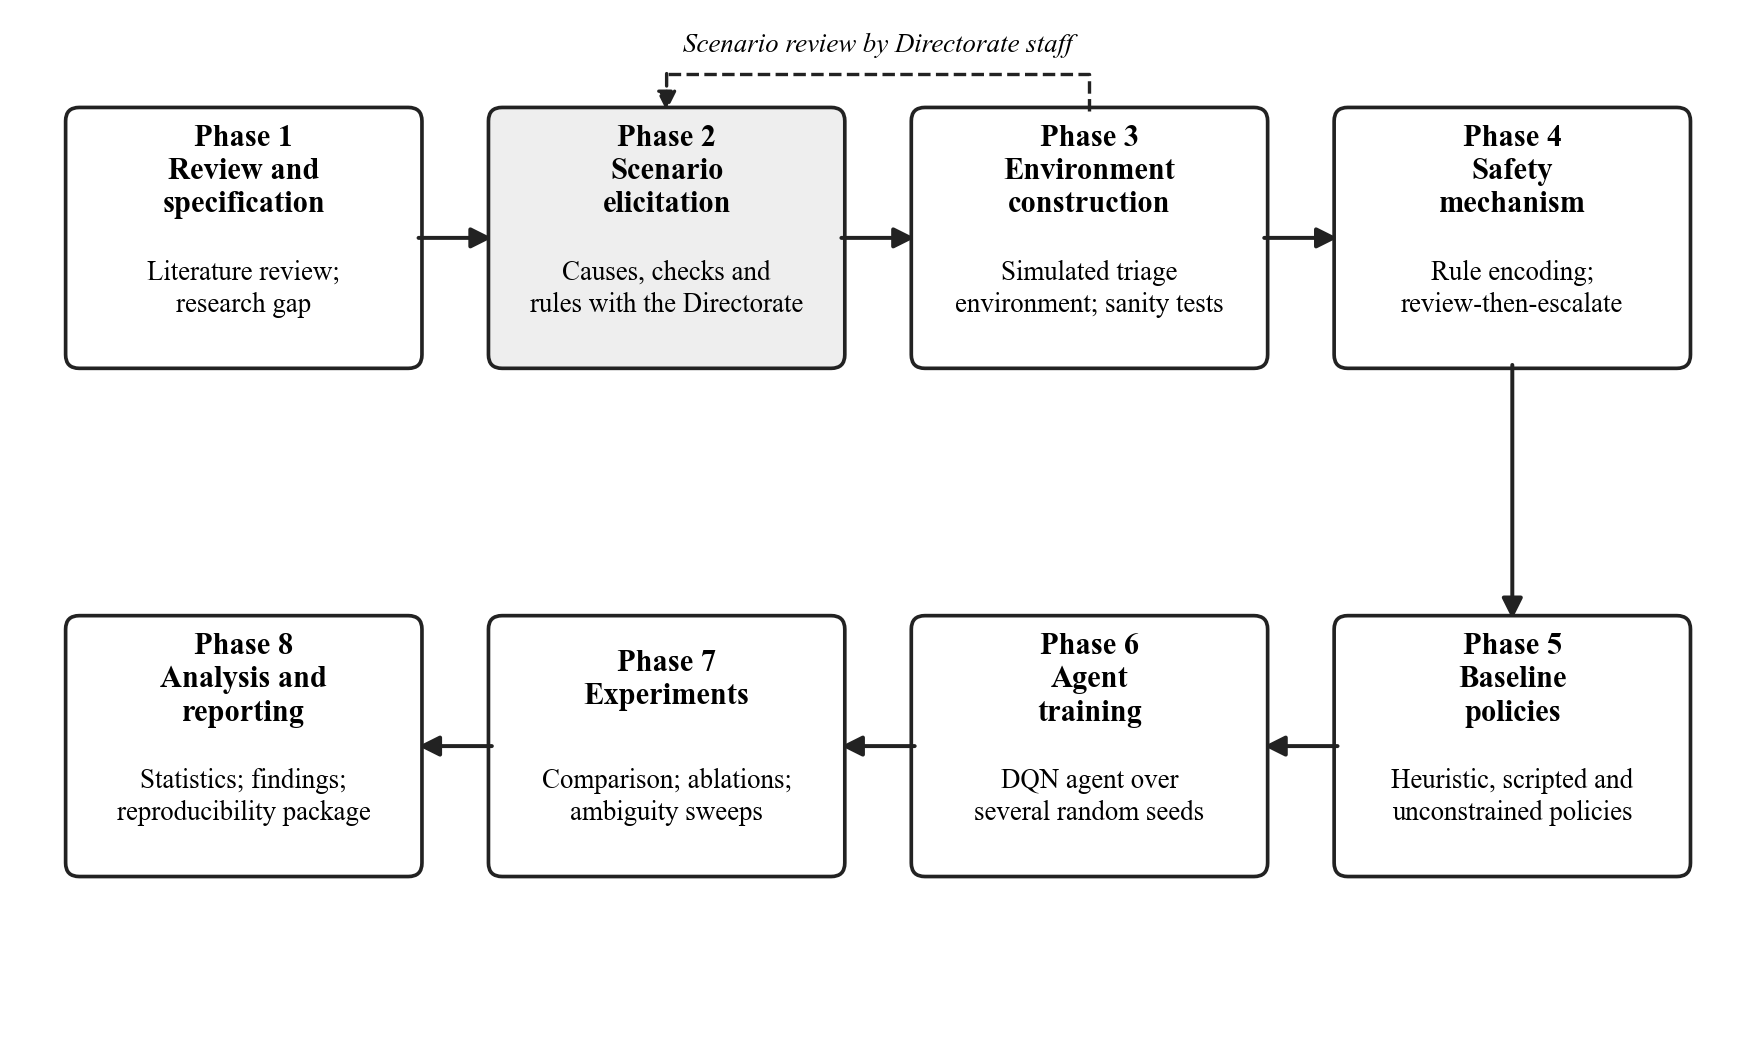
\includegraphics[width=\textwidth]{Figure_3_1_Research_Pipeline.png}
\caption{The research pipeline of the study.}
\label{fig:pipeline}
\end{figure}

The order of the phases reflects their dependencies. The environment cannot be built before the scenarios are specified, and the rules cannot be encoded before the actions and evidence they refer to exist in the environment. The baselines are implemented before the agent is trained so that the environment is exercised by simple policies first, which exposes errors in the simulator before they can be mistaken for properties of the learned agent.

\section{Scenario Modelling with the Directorate}
\label{sec:scenarios}

The scenario model defines what an incident is in the simulation. It consists of about 15 causes, 20 diagnostic checks and 10 operational rules. Fifteen causes is a target, not a limit: more are added if the Directorate can describe them well, since a smaller model that practitioners can rate and review with care is preferred to a larger one whose later entries are guesses. Following the initial consultation, the causes are drawn mainly from application errors observed in the logs of the university's systems, together with infrastructure causes that surface in those logs. They are distributed across four provisional categories: application and interface errors, authentication and access failures, database failures, and failures of infrastructure and external services. The categories are confirmed or revised in the elicitation. Each cause is associated with one remedy, which is the action that resolves an incident with that cause. Each check is a diagnostic observation that a member of IT staff could obtain, such as an entry in the application logs, a value on the monitoring dashboard, the result of reproducing a failing request or the state of a service, and each check has a cost that represents the effort of obtaining it. The symptoms correspond to what is first seen of an incident, such as the type of error and the affected function recorded in the logs, or the category of a user's ticket.

The content of the model is elicited from the Directorate. The elicitation seeks the causes of incidents that the Directorate encounters in these categories and the remedy for each, the symptoms with which those incidents are first reported, the checks that IT staff use to distinguish one cause from another, the rules that govern which actions may be taken and under what conditions, and the attributes of an incident to which those rules refer, such as whether the affected system is in production and the priority of the incident. The symptoms form a fixed list, so that each symptom is a named indicator and not free text. For each pair of cause and check, and for each pair of cause and symptom, the elicitation seeks a judgement of how likely the check or symptom is to be positive when that cause is present. It also seeks the approximate relative frequency of each cause and the effort required by each check. Where the Directorate can offer them, it seeks the relative costs of an escalation and of a wrong remedy and the frequency with which checks are unavailable or misleading; these inform the reward values and the ranges of the ambiguity controls but do not fix them. Any parameter that the elicitation does not supply is set by the researcher and reported as such.

The likelihoods are elicited on a five-point verbal scale, from \emph{never} through \emph{rarely}, \emph{sometimes} and \emph{often} to \emph{almost always}, which is mapped to the probabilities 0.05, 0.25, 0.5, 0.75 and 0.95. Asking for a verbal rating rather than a probability for each of the 300 pairs of cause and check keeps the task manageable for practitioners. Judgements are sought for the pairs that the Directorate considers related, and unrelated pairs take a default value that is reported with the model. The source of each judgement is recorded. These judgements become the parameters of the incident model described in Section~\ref{sec:environment}. The arrangements for the elicitation, including whether it draws on consultation with IT staff, on anonymised counts from the Directorate's ticketing and monitoring systems, or on both, are subject to the agreement reached with the Directorate. Such counts, for example of incidents by type and of the time taken to resolve them, would inform the relative frequency of each cause and the cost of an escalation.

The model is validated by expert review. After the environment has been built, sample incidents generated by the simulator are presented to Directorate staff, who judge whether the combinations of symptoms, check results and causes are plausible and whether the rules are stated correctly. The model is revised in response and then fixed before any agent is trained. Fixing the model before training prevents the scenarios from being adjusted, even unintentionally, in favour of the proposed agent.

The scenario model is a simplification, and the study states its simplifying assumptions. Each incident has exactly one cause, each cause has one correct remedy, and the result of a check does not change during an incident. Symptoms reach the agent as structured indicators from the elicited list; extracting them from the free text of a ticket is outside the scope of the study. These assumptions keep the model small enough to be specified and reviewed by people, at the cost of excluding incidents with several interacting causes and the errors that would arise in reading symptoms from text.

\section{The Simulated Triage Environment}
\label{sec:environment}

The environment casts triage as a sequential decision problem under partial observability. Chapter Two showed that a hidden cause with noisy observations is an established representation of an incident~\cite{kaelbling1998,kim2025,hammar2026belief}. The environment follows that representation and is implemented with the standard interface for reinforcement learning environments~\cite{towers2024}. One episode of the environment corresponds to the triage of one incident.

\subsection{Incident Model}

At the start of an episode the environment draws a cause $c$ from the set of causes $C = \{c_1, \dots, c_{K}\}$, where $K$ is the number of elicited causes (about 15), according to a prior distribution $P(c)$. The cause is hidden from the agent for the whole episode. The environment also draws a context for the incident, consisting of attributes such as whether the affected system is a production system and the priority of the incident. The context is visible to the agent, and the operational rules refer to it.

Evidence about the cause is generated by a likelihood model. Each diagnostic check $d_i$ in the set $D = \{d_1, \dots, d_{20}\}$ has a binary result, and the probability of a positive result depends on the cause:
\begin{equation}
\theta_{ij} = P(d_i = \text{positive} \mid c_j).
\label{eq:likelihood}
\end{equation}
The initial symptoms of the incident are generated in the same way from a set of symptom indicators, and they are revealed to the agent at the first step. The true result of every check is drawn once at the start of the episode, independently of the other checks given the cause, so that requesting a check twice returns the same result.

\subsection{Observations and State}

The agent never observes the cause. It observes an evidence vector that records, for each check, one of four values: not yet requested, unavailable, negative or positive. Each symptom indicator takes one of three values, present, absent or not reported, since all symptoms are revealed at the first step. The vector also contains the context attributes, the number of steps taken, and an indicator that is set when the previous proposal was blocked by the safety mechanism. This evidence vector is the agent's estimate of the incident state. Giving the learner access to the state of the safety mechanism follows Alshiekh et al., whose learner can base its actions on the state of the shield~\cite{alshiekh2018}.

The evidence vector is presented to the agent as a fixed-length vector of numbers. Each categorical value, namely the result of a check, the value of a symptom and each context attribute with more than two levels, is one-hot encoded, so that no artificial ordering is imposed on its values. Binary attributes and the blocked indicator take the values 0 and 1, and the number of steps is divided by the step limit so that it lies between 0 and 1. The length of the vector is fixed by the number of symptoms and context attributes established in the elicitation.

Because the results of checks do not change within an episode, the vector summarises everything the agent has learned about the incident, and the agent does not need a memory of earlier steps. Studies of incident response in which evidence arrives as a stream of events encode a history, with a transformer over recent security events~\cite{ren2025} or with recent telemetry and alert history~\cite{alauthman2026}, and a model of a fatiguing human expert uses a sequence model to track workload over an episode~\cite{zhang2026falcon}. The static evidence assumed here allows a feed-forward network to be used instead.

This choice does not give up the belief that a partially observable formulation requires. In the systematic review, the methods that kept an explicit belief over the hidden state were the most robust to model error and system change~\cite{opol2026slr,hammar2025,hammar2026belief}. In this environment the results of checks are fixed within an episode and independent of one another given the cause, and missing and reversed results arise independently of the cause. The posterior probability of each cause is then determined by the prior, the initial symptoms and the results observed so far, so the evidence vector is a sufficient statistic for the belief that a partially observable agent would maintain~\cite{kaelbling1998}. The agent does not compute that belief explicitly, because it is not given the likelihood model; it must learn the mapping from evidence to action. The threshold policy of Section~\ref{sec:baselines}, which is given the likelihood model and computes the posterior directly, serves as the explicit-belief reference.

\subsection{Actions}

The agent has $20 + K + 1$ actions, 36 with 15 causes. Twenty actions each request one diagnostic check, $K$ actions each recommend the remedy for one cause, and one action escalates the incident to a human expert. A request returns the result of the check and continues the episode. A check that has already been requested is removed from the agent's choices for the rest of the episode, since repeating it would return the same result. A recommendation or an escalation ends the episode. An episode also ends, as an escalation, if the agent reaches a fixed limit on the number of steps without deciding.

\subsection{Reward}

The reward expresses the costs that Chapter One attributed to each choice. A correct recommendation receives a positive reward $r_{\text{correct}}$. A wrong recommendation receives a penalty $-\lambda_{\text{wrong}}$. Each request for check $d_i$ incurs its cost $-k_i$. An escalation incurs a cost $-\lambda_{\text{esc}}$, which represents the expert's time. The values satisfy
\begin{equation}
r_{\text{correct}} > -\lambda_{\text{esc}} > -\lambda_{\text{wrong}},
\label{eq:reward}
\end{equation}
so that resolving an incident correctly is better than escalating it, and escalating it is better than recommending the wrong remedy. The simulated expert is assumed to resolve every escalated incident. The numerical values are set in pilot runs before the experiments begin and are reported with the results. Because the behaviour of the agent depends on these values, the study also examines how the results change when the cost of escalation is varied.

\subsection{Ambiguity Controls}
\label{sec:ambiguity}

Chapter Two identified three sources of ambiguity: missing observations, unreliable observations, and observations consistent with more than one cause. The environment has one control for each.

\begin{enumerate}
  \item \textbf{Missing evidence.} With probability $p_{\text{miss}}$, a check is unavailable for the whole episode, and a request for it returns the value ``unavailable''.
  \item \textbf{Unreliable evidence.} With probability $p_{\text{noise}}$, the result of a check is reversed before the agent receives it.
  \item \textbf{Overlapping evidence.} An overlap parameter $\omega$ between 0 and 1 moves the likelihood profile of each cause towards the average profile of its category, $\theta'_{ij} = (1 - \omega)\,\theta_{ij} + \omega\,\bar{\theta}_{i}$, where $\bar{\theta}_{i}$ is the mean of $\theta_{ij}$ over the causes in the same category as $c_j$. As $\omega$ increases, causes within a category become harder to tell apart.
\end{enumerate}

A setting of the three controls defines an ambiguity level. The base level, used for training and for the main comparison, is fixed in pilot runs so that the task is neither trivial nor impossible. The planned ranges for the robustness experiment are $p_{\text{miss}} \in \{0, 0.2, 0.4, 0.6\}$, $p_{\text{noise}} \in \{0, 0.1, 0.2, 0.3\}$ and $\omega \in \{0, 0.25, 0.5, 0.75\}$.

\subsection{Reference Labels}
\label{sec:labels}

The simulator knows the hidden cause and the likelihood model, so it can label each episode with the outcome that would have been appropriate. An incident is labelled as one that should be escalated in either of two cases. In the first, the operational rules prohibit the agent from recommending the remedy for the true cause in the context of the incident. In the second, the incident is irreducibly ambiguous: even with the result of every available check, the most probable cause under the simulator's own model is not the true cause. All other incidents are labelled as resolvable. These labels are used only for evaluation and are never shown to the agent.

The simulator is checked for leakage of the hidden cause before any agent is trained. Sahin and Mert found that an earlier version of their own simulator leaked the label into the agent's observations, so that any threshold appeared to achieve perfect recall~\cite{sahin2026}. In this environment no policy that sees only the observations can, on average, resolve correctly a larger share of incidents than the recommendation of the most probable cause after every available check, and by the definition above that share is the share of incidents labelled as resolvable. This ceiling is computed at each ambiguity level, and a learned or baseline policy whose resolution accuracy exceeds it by more than sampling error is taken as evidence of leakage, to be corrected before the experiments proceed.

\section{The Reinforcement Learning Agent}
\label{sec:agent}

The agent learns a policy that maps the evidence vector to one of the $20 + K + 1$ actions. The primary learning algorithm is the deep Q-network (DQN), which estimates the expected return of each action with a neural network~\cite{mnih2015}. Three considerations motivated the choice. First, the action set is small and discrete, which value-based methods handle directly. Second, the evidence vector admits $4^{20}$ combinations for the checks alone, which rules out the tabular Q-learning used in earlier incident-handling and shielding studies~\cite{dunsin2025,alshiekh2018} while retaining the same family of methods. Third, DQN yields an estimated value for every action, so the values the agent assigns to a blocked remedy and to escalation can be inspected when its behaviour is analysed. Constrained optimisers such as constrained policy optimisation and PPO-Lagrangian~\cite{achiam2017,zhang2026falcon} were not adopted, because they bound the expected cumulative cost of a policy, whereas the operational rules must hold at every step and are enforced by a separate mechanism (Section~\ref{sec:mechanism}). Policy-gradient methods are common in recent shielding studies~\cite{yang2023,konighofer2025}, and proximal policy optimisation~\cite{schulman2017} therefore serves as a secondary learner. Where time permits, the main comparison is repeated with it to show whether the findings depend on the choice of learner. Both algorithms are taken from an established open-source library to limit implementation error~\cite{raffin2021}. The library's DQN does not support action masking, so the removal of blocked actions and of checks already requested is implemented by restricting the choice of action, and the maximum in the learning target, to the available actions.

Each agent is trained by interaction with the environment at the base ambiguity level. Training begins from the library's default hyperparameters, and a small search over the learning rate, the network size and the exploration schedule is carried out on a set of random seeds that is not used in the final experiments. The training length is set from the pilot runs as the point at which the mean return stops improving. The final hyperparameters, the training length and the search itself are reported with the results.

A second training regime is used for the robustness question. In it the ambiguity controls are drawn at random from their planned ranges at the start of each episode, so that the agent meets many levels of ambiguity during training. Comparing the two regimes shows whether robustness requires exposure to ambiguity during training or carries over from training at a single level.

\section{The Rule-Based Safety Mechanism}
\label{sec:mechanism}

The safety mechanism is a component separate from the agent that checks every proposed action against the operational rules. Each rule is a condition over three things: the proposed action, the context of the incident, and the evidence gathered so far. A rule may, for example, prohibit a remedy on a production system, or prohibit a remedy until a named check has been observed. An action is prohibited if any rule prohibits it. Escalation is never prohibited, so a permitted action always exists. The ten rules are those elicited from the Directorate, encoded as explicit conditions that can be read and reviewed without reference to the agent.

The mechanism follows a review-then-escalate procedure when it blocks a proposal.

\begin{enumerate}
  \item The agent proposes an action. If no rule prohibits it, the action passes to the environment unchanged.
  \item If a rule prohibits the action, the mechanism blocks it and records the event. The step is consumed without reward. The agent receives the same evidence vector with the blocked indicator set, and the blocked action is removed from its choices for the next step.
  \item The agent proposes a second action. If it is permitted, it passes to the environment and the episode continues as normal.
  \item If the second proposal is also prohibited, the mechanism ends the episode by escalating the incident to the human expert. This outcome is recorded as a forced escalation.
\end{enumerate}

This design responds to three findings of Chapter Two. The first is that its central step has no precedent: of the 34 studies in the systematic review, only three report what replaces a blocked decision, by substitution, hand-off or deferral, and none gives the agent a second proposal~\cite{opol2026slr,ravi2025,singh2026,sahin2026}. The other two concern how the block is handled. A shield that silently replaces an action can hinder learning because the agent does not know that it was overridden~\cite{yang2023}; here the agent is told of the block and given one opportunity to choose again. Where a decision cannot be made within the rules, the appropriate fallback is to hand it to a person~\cite{pacella2026}; here a second block has that effect. The mechanism belongs to the family of shields that act after the agent has chosen~\cite{alshiekh2018}. It differs from them in that its rules are written directly and not synthesised from a formal model of the environment, so it carries no formal guarantee beyond the rules as written. Within the simulation it ensures that no prohibited action is executed.

\section{Baseline Decision Policies}
\label{sec:baselines}

No published system can be compared with the proposed agent directly, because the closest studies address other domains and share no environment with this one. The agent is therefore compared with baseline policies that run in the same environment, each standing for an approach identified in Chapter Two. Table~\ref{tab:baselines} lists them.

\begin{table}[htbp]
\centering
\caption{Baseline decision policies and the approaches they represent.}
\label{tab:baselines}
\small
\begin{tabularx}{\textwidth}{@{}p{0.2\textwidth}LL@{}}
\toprule
Policy & Behaviour & Approach represented \\
\midrule
Initial-symptom policy & Recommends the most probable cause given the initial symptoms, without requesting checks & Triage as a single prediction~\cite{chen2020,remil2024} \\
Scripted policy & Requests a fixed sequence of checks for the reported category and then recommends the most probable cause & Rule-based and runbook practice~\cite{remil2024,dantonio2025} \\
Always-escalate policy & Escalates every incident & The limiting case of deferral \\
Threshold policy & Maintains the posterior probability of each cause, requests the most informative check while no cause exceeds a confidence threshold, recommends when one does, and escalates when the checks are exhausted & Selective prediction and uncertainty-driven investigation~\cite{geifman2019,kim2025} \\
Unconstrained agent & The same learning agent trained and run without the safety mechanism & The standard comparison in shielding studies~\cite{alshiekh2018,jansen2020} \\
Penalty-only agent & The same learning agent without the mechanism, with a reward penalty for each prohibited action & Constraint by reward penalty~\cite{konighofer2025} \\
\bottomrule
\end{tabularx}
\end{table}

The order of checks in the scripted policy is elicited from the order in which Directorate staff examine evidence for each category of incident, so that the policy reflects current practice and not an arbitrary sequence. This matters because, in the systematic review, no extracted result showed a static baseline outperforming a learned policy, and weak baselines could not be ruled out as the reason~\cite{opol2026slr}. Where the elicitation does not supply an order for a category, the checks are ordered by their expected information about the cause under the elicited likelihoods, and this is reported.

Two of these baselines deserve comment. The threshold policy is given the simulator's likelihood model, which the learning agent must infer from experience. It is therefore a strong reference, and the study does not assume that the learned agent will exceed it. The always-escalate policy executes no prohibited action and makes no wrong recommendation, and it shows why no single measure can be read alone. The first four policies are run with the safety mechanism in place, so that their proposals are checked in the same way as those of the proposed agent.

Two ablations of the proposed agent complete the comparison. In the first, the agent cannot request checks and must recommend or escalate from the initial symptoms, which corresponds to the two-way choice studied in the deferral literature~\cite{madras2018}. In the second, the agent cannot escalate voluntarily and must gather evidence and then recommend, which corresponds to the two-way choice studied in the literature on information acquisition~\cite{janisch2019}. The ablations show what each option contributes to the three-way decision.

\section{Evaluation Metrics}
\label{sec:metrics}

Every policy is evaluated on the same fixed set of $N$ evaluation episodes at each ambiguity level. Each episode ends in a correct recommendation, a wrong recommendation or an escalation. Let $N_{\text{c}}$, $N_{\text{w}}$ and $N_{\text{e}}$ be the numbers of episodes with each outcome, so that $N = N_{\text{c}} + N_{\text{w}} + N_{\text{e}}$. The metrics are standard measures taken from the strands of literature reviewed in Chapter Two, and they are grouped under the four measures named in the fourth objective.

\subsection{Decision Quality}

Decision quality describes how often the agent's final decision is right. \emph{Resolution accuracy} is the share of all incidents that the agent resolves itself, $N_{\text{c}} / N$. It is the usual accuracy of the triage literature~\cite{remil2024}, and it penalises an agent that avoids error by escalating. \emph{Coverage} is the share of incidents on which the agent makes a recommendation, $(N_{\text{c}} + N_{\text{w}}) / N$, and \emph{selective accuracy} is the accuracy of those recommendations, $N_{\text{c}} / (N_{\text{c}} + N_{\text{w}})$. These two are the standard pair of selective prediction~\cite{geifman2019}. They are reported together because either can be raised at the expense of the other. The \emph{wrong-recommendation rate}, $N_{\text{w}} / N$, isolates the most costly error in triage. The \emph{mean episodic return} is the average total reward per episode. It is the quantity the agent is trained to maximise and the standard summary in reinforcement learning~\cite{sutton2018}, but it depends on the reward values chosen and is never reported alone.

\subsection{Investigation Efficiency}

Investigation efficiency describes what the agent spends on evidence before it decides. The \emph{mean number of checks} is the average number of requests per episode, and the \emph{mean investigation cost} is the average of the summed check costs per episode. The cost stands in for time, which a simulation without a clock cannot measure directly. The two are read together with accuracy as an \emph{accuracy--cost curve}, following the evaluation of costly feature acquisition~\cite{janisch2019}. The curve shows whether additional investigation yields additional accuracy and allows policies to be compared at equal cost.

\subsection{Escalation Behaviour}

Escalation behaviour describes how much the agent hands to the human expert and whether it hands over the right cases. The \emph{escalation rate} is $N_{\text{e}} / N$, the load placed on human experts~\cite{turan2026}. The remaining metrics use the reference labels of Section~\ref{sec:labels}. \emph{Escalation precision} is the share of escalated incidents that were labelled as ones that should be escalated; low precision means that human experts receive incidents the agent could have resolved. \emph{Escalation recall} is the share of incidents labelled as ones that should be escalated that the agent did escalate; low recall is the failure of under-escalation that Pacella et al.\ measured~\cite{pacella2026}. The \emph{escalation F1 score} is the harmonic mean of the two. Because precision, recall and F1 can all look acceptable when one class is rare, the \emph{escalation Matthews correlation coefficient} between the agent's choice to escalate and the reference label is also reported; it uses all four cells of the confusion matrix, and Okafor found that it exposed degenerate triage policies that F1 and ROC-AUC concealed~\cite{okafor2026}. Forced escalations are excluded from these three metrics and reported under constraint compliance, because they are produced by the mechanism and not chosen by the agent. Escalations caused by the step limit are likewise counted separately.

\subsection{Constraint Compliance}

Constraint compliance describes the agent's relationship to the rules. The \emph{proposed-violation rate} is the number of blocked proposals divided by the number of proposals. It shows whether the agent has learned to act within the rules or relies on being stopped. The \emph{forced-escalation rate} is the share of episodes that end with a second blocked proposal. The \emph{executed-violation rate} is the share of episodes in which a prohibited action takes effect. It is zero by construction when the mechanism is active, and it is the central measure for the unconstrained and penalty-only agents, as in the shielding literature~\cite{alshiekh2018,jansen2020}. The \emph{compliant success rate} is the share of episodes that end in a correct recommendation with no executed violation. It follows the measure of completion under policy introduced for agent benchmarks~\cite{levy2026}, and for agents without the mechanism it shows how much of their accuracy was obtained by breaking rules.

\subsection{Robustness}

Robustness is not a separate metric. Each metric above is computed at every ambiguity level and reported as a function of that level, in the manner of studies that vary false-alert rates or model error~\cite{kim2025,hammar2025}. Two views are reported. The first is degradation, the change in resolution accuracy and wrong-recommendation rate relative to the base level. The second is the decision mix, the coverage, the escalation rate and the mean number of checks at each level, which shows whether the agent responds to ambiguity by investigating more, by escalating more, or by continuing to recommend on weaker evidence.

\section{Experimental Design}
\label{sec:experiments}

The study comprises four experiments. Each learning agent is trained with ten random seeds, and results are reported as the mean over seeds with a 95\% bootstrap confidence interval, following recommended practice for reporting reinforcement learning results~\cite{agarwal2021}. The evaluation episodes are generated with seeds that are not used in training, and the same episodes are presented to every policy so that differences between policies are not due to differences between incidents. These choices answer the reporting weaknesses found in the systematic review, in which only 11 of 34 studies reported results over several runs with a measure of variance, nine tested their agents on conditions not seen in training, and five reported their hyperparameters and released their code or environment~\cite{opol2026slr}. This study reports variance over seeds, evaluates on unseen episodes and on ambiguity levels not used in training, and archives its code and configurations (Section~\ref{sec:tools}).

\textbf{Experiment 1: comparison with baselines.} The proposed agent is compared with the six baseline policies at the base ambiguity level on all metrics. This experiment addresses the fourth research question and the first hypothesis.

\textbf{Experiment 2: effect of the safety mechanism.} The proposed agent is compared with the unconstrained agent and the penalty-only agent on the constraint compliance metrics and on decision quality, and the proposed-violation rate is tracked over training. The two studies in the systematic review that measured a hard rule mechanism reached opposite results, one finding that the rules cost almost nothing~\cite{singh2026} and the other that they produced many false actions~\cite{ravi2025}, and neither reported how often blocked proposals occurred as training progressed. Tracking that rate shows whether the agent learns to act within the rules or continues to rely on being stopped. This experiment addresses the third research question and the second hypothesis.

\textbf{Experiment 3: ablation of the action set.} The proposed agent is compared with its two ablations to establish what the options to investigate and to escalate each contribute. This experiment addresses the second research question.

\textbf{Experiment 4: robustness.} All policies are evaluated across the planned ranges of the three ambiguity controls, varied one at a time from the base level and then jointly, for agents trained under both training regimes. This experiment addresses the fifth research question and the third hypothesis.

The first research question, on representation, is answered by the scenario model and the environment themselves and by their review by Directorate staff. A sensitivity analysis accompanies the experiments: the cost of escalation is varied around its chosen value and Experiment 1 is repeated, to show how far the conclusions depend on the reward design.

\section{Tools and Implementation}
\label{sec:tools}

The environment, the safety mechanism and the baselines are implemented in Python. The environment follows the Gymnasium interface~\cite{towers2024}, and the learning algorithms are those of Stable-Baselines3~\cite{raffin2021}. The scenario model, the rules and the settings of every experiment are held in configuration files and not in code, so that each result can be traced to the configuration that produced it. Random seeds are fixed and recorded. The code, the configurations and the evaluation episodes will be archived with the project so that the experiments can be repeated, with any material that the Directorate regards as confidential withheld or generalised.

\section{Validity and Limitations}
\label{sec:validity}

The main threat to the validity of the study is the realism of the simulator. The agent's behaviour is valid for incidents generated by the likelihood model, and that model rests on elicited judgements and on the simplifying assumptions of Section~\ref{sec:scenarios}. Expert review of generated incidents reduces this threat but does not remove it. The findings should therefore be read as evidence about the method under stated assumptions, and not as a prediction of performance on live incidents.

Three further limitations follow from design choices. First, the simulated expert resolves every escalated incident at a fixed cost. Chapter Two showed that the accuracy of human reviewers varies with workload~\cite{zhang2026falcon,turan2026}, so the study understates the cost of heavy escalation, and it reports the escalation rate so that this cost remains visible. Second, the results depend on the reward values, which the sensitivity analysis addresses only for the cost of escalation. Third, the safety mechanism enforces the rules as written, and it can only evaluate a rule on the evidence available; a rule that depends on a fact the agent has not observed cannot be applied correctly~\cite{wugong2026}.

The study also limits what it claims about generality. The scenario model reflects the practice of one organisation and four categories of incident, and the initial consultation drew on a single interview. Whether the findings hold for other organisations, other categories or larger models is a question for further work.

\section{Ethical Considerations}

The study will be conducted with the permission of the Directorate and in accordance with the research ethics requirements of the university. Participation by Directorate staff in the interviews, elicitation and review is voluntary, consent is obtained before any statement is used, and no member of staff is identified in the report. The initial consultation identified the security of incident data, including control over who can see it, as the main condition for using an agent of this kind; this is one reason the study works from elicited parameters in simulation and not from live data. Any incident records used to inform the scenario model are anonymised before use, and no personal data, credentials or confidential details of the university's systems appear in the simulator, the report or the archived materials. The agent is trained and evaluated only in simulation. It is not connected to any live system, and it executes no action on the infrastructure of the university.

\section{Chapter Summary}

This chapter described the methodology of the study. The study constructs a simulated triage environment from a scenario model of about 15 causes, 20 diagnostic checks and 10 operational rules elicited from the Directorate of University ICT Services, in which missing, unreliable and overlapping evidence can each be controlled. A reinforcement learning agent chooses among requesting checks, recommending remedies and escalating, and an independent rule-based mechanism reviews each proposal, returns a blocked proposal to the agent once, and escalates the incident if the second proposal is also blocked. The agent is compared with six baseline policies and two ablations on standard measures of decision quality, investigation efficiency, escalation behaviour and constraint compliance, across controlled levels of ambiguity. Chapter Four presents the implementation and the results of these experiments.
